\documentclass[12pt]{article}

% PACKAGES

\usepackage[
top=2.50cm,
bottom=2.50cm,
left=2cm,
right=2cm,
marginparsep=0pt,
marginparwidth=0pt]{geometry}
\usepackage{fancyhdr}
\usepackage{float}
\usepackage{dirtree}
\usepackage{cancel}
\usepackage{mathtools}
\usepackage{amsmath}
\usepackage{amsthm}
\usepackage{amssymb}
\usepackage{textcomp}
\usepackage{ulem}
\usepackage{verbatim}
\usepackage{contour}
\usepackage{graphicx}
\usepackage{svg}
\usepackage{xcolor}
\usepackage[T1]{fontenc}
\usepackage{inputenc}
\usepackage[utf8]{inputenx}
\usepackage[unicode]{hyperref}
\usepackage[shortlabels]{enumitem}
\usepackage{booktabs}
\usepackage{bookmark}
\usepackage{listings}
\usepackage{xcolor}
\usepackage{tocloft}
\usepackage{tikz}
\usepackage{xspace}
\usepackage[most]{tcolorbox}

% MACROS & DEFS

\newcommand{\modelmapper}{\texttt{modelmapper}\xspace}

\newcommand{\floor}[1]{\left\lfloor #1 \right\rfloor}
\newcommand{\ceil}[1]{\left\lceil #1 \right\rceil}
\newcommand{\round}[1]{\left\lfloor #1 \right\rceil}
\newcommand{\abs}[1]{\left\lvert #1 \right\rvert}

\DeclareRobustCommand{\ul}[1]{%
	\uline{\phantom{#1}}%
	\llap{\contour{white}{#1}}%
}

\renewcommand{\ULdepth}{1.8pt}
\contourlength{0.8pt}

\setlength{\parindent}{0em}
\setlength{\parskip}{0.75em}

\definecolor{codegreen}{RGB}{0,135,0}
\definecolor{codegray}{RGB}{135,135,135}
\definecolor{codemagenta}{RGB}{215,0,135}
\definecolor{codepurple}{RGB}{135,0,175}
\definecolor{backcolour}{RGB}{238,238,238}

\definecolor{bookyellow}{RGB}{255,255,224}

\DeclareTotalTCBox{\shell}{ O{black} v !O{} }
{
    fontupper=\ttfamily,
    nobeforeafter,
    tcbox raise base,
    arc=0pt,
    outer arc=0pt,
    top=0.1mm,
    bottom=0.1mm,
    left=0.1mm,
    right=0.1mm,
    leftrule=0pt,
    rightrule=0pt,
    toprule=0.3mm,
    bottomrule=0.3mm,
    boxsep=0.5mm,
    colback=#1!60!white,
    colframe=#1!70!black,
    #3
}{\textcolor{white}{#2}}

% PACKAGE CONFIG

\lstdefinestyle{code}{
	basicstyle=\ttfamily\small,
	commentstyle=\color{codegray}\itshape,
	keywordstyle=\color{codepurple},
	stringstyle=\color{codegreen},
	aboveskip=25pt,
    belowskip=10pt,
	captionpos=b,
	abovecaptionskip=12.5pt,
	breaklines=true,
	numbers=none,
	frame=tb,
	framesep=5pt,
	keepspaces=true,
	showspaces=false,
	showstringspaces=false,
	breakatwhitespace=false,
	tabsize=2,
	showtabs=false,
}

\lstset{style=code}

% Set dots for table of contents
\renewcommand{\cftdot}{.}
\renewcommand{\cftsecleader}{\cftdotfill{\cftdotsep}}

% Set theorem
\newtheorem*{definition}{Definition}

% HEADER & FOOTER

\setlength{\headheight}{15pt}
\pagestyle{fancy}
\renewcommand{\headrulewidth}{0pt}
\lhead{J. Scerri}
\chead{CPS2002 --- Code Analysis}
\rhead{\thepage}

% TITLE

\title{CPS2002 --- Code Analysis\\
\vspace{1em}\textbf{Assignment Part 2}}

\date{\today}

\author {{\textbf{Juan Scerri}}\\
B.Sc. (Hons)(Melit.) Computing Science and Mathematics (Second Year)}

\begin{document}

%----------------------------------
%	TITLE PAGE
%----------------------------------

\maketitle % Print the title page

\thispagestyle{empty} % Suppress headers and footers on the title page

%----------------------------------

\tableofcontents

\clearpage

\listoffigures

\lstlistoflistings

\clearpage

\section{Plagiarism Declaration}

Plagiarism is defined as \textit{``the unacknowledged use, as
one's own, of work of another person, whether or not such work
has been published, and as may be further elaborated in Faculty
or University guidelines''} (\ul{University Assessment
Regulations}, 2009, Regulation 39 (b)(i), University of Malta).

I, the undersigned, declare that the report submitted is my
work, except where acknowledged and referenced. I understand
that the penalties for committing a breach of the regulations
include loss of marks; cancellation of examination results;
enforced suspension of studies; or expulsion from the degree
programme.

Work submitted without this signed declaration will not be
corrected, and will be given zero marks.

\vfill

\begin{minipage}[t]{0.3\textwidth}
\ul{Juan Scerri} \medskip

\textbf{Student's full name} \medskip
\end{minipage}
\hfill
\begin{minipage}[t]{0.3\textwidth}
\ul{CPS2002} \medskip

\textbf{Study-unit code} \medskip
\end{minipage}
\hfill
\begin{minipage}[t]{0.3\textwidth}
\ul{{\today}} \medskip

\textbf{Date of submission} \medskip
\end{minipage}

\vspace{2cm}

\textbf{Title of submitted work:} \ul{CPS2002 Code Analysis}

\vspace{2cm}

\textbf{Student's signature} \medskip

\underline{
\includegraphics[height=2cm]{images/sig.png}}
\medskip

\section{Selected Open--Source Project}

The selected open--source project which will be analysed in this
report is the \modelmapper project. It is a simple Java library
which allows for the conversion of a class into another (see
listing \ref{modemapper-usage}).

\begin{lstlisting}[language=Java, caption={Using the
\modelmapper library}, label={modelmapper-usage}]
public class PersonEntity {
    public Id id;
    public String name;
    public String surname;
    public int age;

    // getter and setters
}

public class Person {
    public Id id;
    public String name;
    public String surname;
    public int age;

    // getter and setters
}

Person person = (new ModelMapper()).map(personEntity, Person.class);
\end{lstlisting}

At the time of writing the project has $721$ commits, $220$ open
issues and $11$ open pull requests. The project was clone from
GitHub and since the project uses Maven, the test suite was ran
with the command \shell{mvn clean test},
(see figure \ref{running-test-suite}).

Furthermore, the test suite was run from within IntelliJ to get
code coverage metrics (see figure \ref{intellij-code-coverage})

\begin{figure}[H]
    \centering
    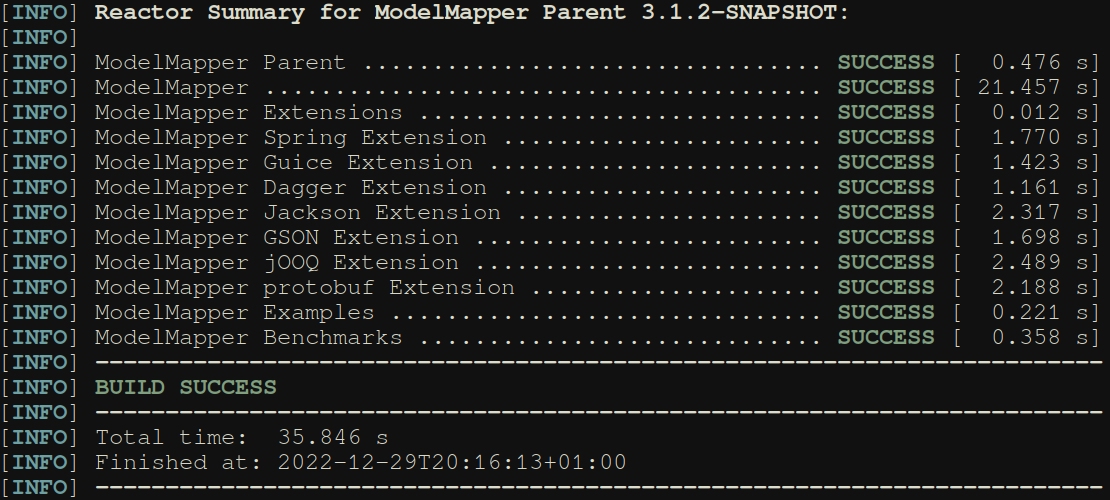
\includegraphics[width=14cm]{images/test-suite.png}
    \caption{Running the test suite}
    \label{running-test-suite}
\end{figure}

\begin{figure}[H]
    \centering
    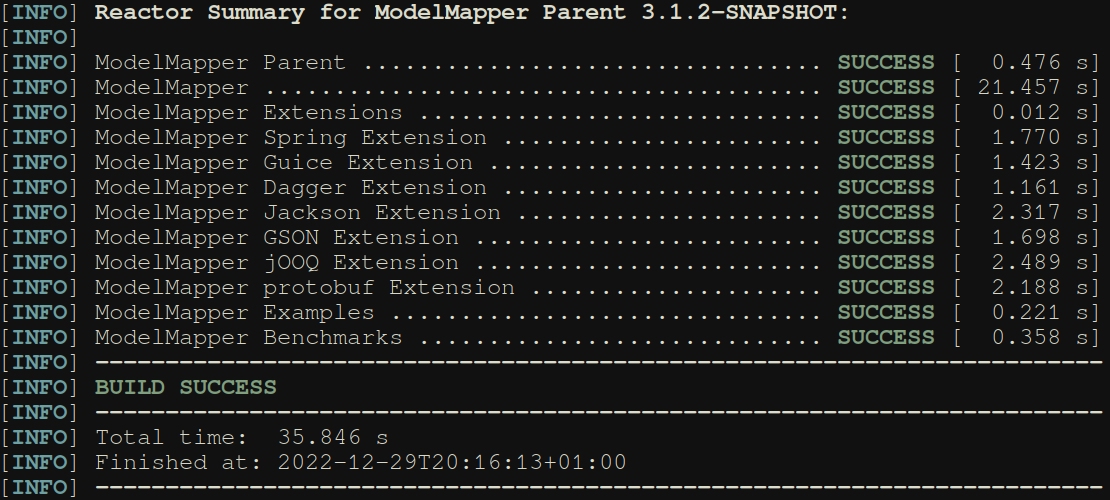
\includegraphics[width=14cm]{images/test-suite.png}
    \caption{Running the test suite}
    \label{intellij-code-coverage}
\end{figure}

\section{Project Analysis}

\subsection{OOP Metrics}

\subsection{Test Suite Suitability}

\subsection{Maintainability}

\end{document}
